%\documentclass[12pt,a4paper]{article}
\documentclass[12pt]{scrartcl}

\KOMAoptions{draft=true}
\KOMAoptions{titlepage=false}
\KOMAoptions{abstract=true}
\KOMAoptions{listof=totoc}

\usepackage[utf8]{inputenc}
\usepackage[T1]{fontenc}
\usepackage[english,ngerman]{babel}

\usepackage{csquotes}
\usepackage{scrhack}
\usepackage[%
    backend=biber,
    style=numeric,
]{biblatex}
\bibliography{literature.bib}
\usepackage[toc,page]{appendix}
\renewcommand{\appendixtocname}{Anhänge}
\renewcommand{\appendixpagename}{Anhänge}
\usepackage{amsmath}
\usepackage{amsfonts}
\usepackage{amssymb}
\usepackage{graphicx}
\usepackage[hidelinks]{hyperref}
\usepackage[locale=DE,binary-units]{siunitx}
\usepackage{algorithm}
\usepackage{algpseudocode}
\floatname{algorithm}{Algorithmus}
\renewcommand{\algorithmicrequire}{\textbf{Input:}}
\renewcommand{\algorithmicensure}{\textbf{Output:}}
\usepackage{listings}
\usepackage[usenames,dvipsnames]{xcolor}


\begin{document}

\begin{titlepage}
    \begin{center}
        {\titlefont\huge Neugengo\par}

        \bigskip
        \bigskip

        {\titlefont\Large --- Praktikumsbericht ---\par}

        \bigskip
        \bigskip

        {\large Arbeitsbereich Wissenschaftliches Rechnen\\
        Fachbereich Informatik\\
        Fakultät für Mathematik, Informatik und Naturwissenschaften\\
        Universität Hamburg\par}
    \end{center}

    \bigskip
    %platz für bild
    \bigskip

    \vfill

    {\large \begin{tabular}{ll}
        Vorgelegt von: & Lennart Braun, Armin Schaare, \\
                       & Theresa Eimer \\
        Betreuer: & Julian Kunkel \\
        \\
        Hamburg, den 30.09.2015
    \end{tabular}\par}
\end{titlepage}

\section*{Abstract}
\thispagestyle{empty}
TODO:


\clearpage

%\renewcommand{\contentsname}{Inhalt}
\tableofcontents

\clearpage

\section{Die Idee}
%Was es tun soll, wieso wir das machen, eine kurze Einleitung eben
Neuronale Netze wurden in den letzten Jahren immer wieder für verschiedene
Problemstellungen benutzt. Es wurde festgestellt, dass sie auch komplizierte
Aufgaben lösen können, vorausgesetzt sie werden gut genug trainiert. Go zu
spielen ist ein sehr komplexe Aufgabe, die wir unter anderem genau aus diesem
Grund ausgewählt haben. Wegen der vielen Zugmöglichkeiten und dem mit 19x19
Punkten sehr großen Spielbrett, gibt es für Go noch keine Computer, die
Menschen deutlich übertreffen oder sogar eine perfekte Strategie spielen
können. Dieses Ziel wäre natürlich etwas hoch gegriffen, doch mit diesem
Projekt wollten wir sehen, ob sich neuronale Netze überhaupt gegenseitig so
trainieren können, dass sie bessere Ergebnisse erzielen. Dazu wurden zwei Tools
benutzt, das erste ist dafür zuständig die Netze zu erstellen und mit Hilfe von
Supervised Learning auf die Regeln von Go zu trainieren. Das zweite Tool lässt
die Netze dann gegeneinander antreten und rekombiniert sie mit Hilfe eines
genetischen Algorithmus. Die so entstandenen Netze können gespeichert werden
und auch gegen einen menschlichen Gegner antreten.

\section{Über Go}
%Kurze Beschreibung der Regeln und unsere Umsetzung
Go ist ein asiatisches Brettspiel, das normalerweise auf Brettern von $19
{\times} 19$ oder $9 {\times} 9$ Schnittpunkten gespielt wird. Es gibt zwei
Spieler, einer spielt schwarze, der andere weiße Steine. Nacheinander legt
zuerst der schwarze, dann der weiße Spieler, je einen Stein auf einen
Schnittpunkt. Ist ein Stein umzingelt, sind also alle seine vier direkt
angrenzenden Schnittpunkte von gegnerischen Steinen besetzt, so ist er
geschlagen und wird vom Brett genommen. Zusammen mit dem auf die selbe Weise
umzingelten Gebiet am Ende des Spieles, bilden die geschlagenen Steine die
Punktzahl der Spieler. Wer mehr Punkte hat gewinnt. Eine Sonderregel ist hier
das Ko. Es ist möglich in eine Endlosschleife zu geraten, indem ein Stein immer
wieder geschlagen und zurückgeschlagen wird. Damit das nicht passiert, darf in
dieser Situation nicht sofort zurückgeschlagen werden, sondern erst einen Zug
später um dem Gegner die Möglichkeit zu geben die Lücke zu schließen. 

Um das Spiel etwas zu vereinfachen und schneller Ergebnisse zu sehen, arbeiten
wir mit $9 {\times} 9$-Spielbrettern. Außerdem gibt es ein Zuglimit für die
Spiele, damit es keine Endlosschleifen gibt, die trotz Ko auftreten können.
Ansonsten haben wir uns aber bemüht die Go Regeln möglichst gut umzusetzen,
damit die Spielstärke auch realistisch beurteilt werden kann.

\section{Unser Programm}

\subsection{Die einzelnen Bereiche}

\subsubsection{Das neuronale Netz}
%Der Aufbau des Netzes, Funktionsweise von Backpropagtion

Ein neuronales Netz besteht aus Neuronen, ähnlich einem menschlichen Gehirn. Die
Neuronen sind in Schichten angeordnet, den Layern des Netzes. Das erste Layer
ist dabei das Input Layer, das letzte das Output Layer. Zwischen den Layern
gehen Kanten von jedem Neuron des einen zu jedem Neuron des anderen Layers.
Diese Kanten haben Gewichte und pro Layer gibt es auch einen Bias, der zum
Kantengewicht addiert wird. Ein Signal wird durch das Input Layer aufgenommen,
durch die Layer weitergegeben und vom Output Layer wieder ausgegeben. Das
Weiterleiten innerhalb des Netzes funktioniert über die Kanten. Der Output eines
Neurons ist die Summe aller seiner Eingänge. Durch eine Sigmoidfunktion, hier
$\frac{1}{1 + e^{-x}}$, werden diese Summen auf den Wertebereich $[-1;1]$
reduziert und gleichzeitig ermöglicht diese Funktion die spätere Anwendung des
Backpropagation Algorithmus, da sie differenzierbar ist. Der fertige Output des
Neurons wird dann mit den jeweiligen Kantengewichten multipliziert und an die
Neuronen des nächsten Layers weitergeleitet. Vor allem hier ist also sehr viel
zu Berechnen. 

Der Aufbau der Netze ist variabel, die Anzahl der Layer sowie die Anzahl der
Neuronen pro Layer ist frei wählbar. Das Input Layer sollte allerdings für jeden
Schnittpunkt des Eingabebrettes ein Neuron haben und das Output Layer
entsprechend ein Neuron pro Schnittpunkt plus ein Neuron um Passen anzuzeigen.
Die Ausgabe sind die Präferenzen der Netze, der Schnittpunkt mit dem höchsten
Wert wird besetzt. 

Damit die Netze zumindest die Regeln von vornherein erlernen, gibt es eine
Methode für Supervised Learning, überwachtes Lernen, den Backpropagation
Algorithmus. Für ihn muss bekannt sein, was das erwartete Ergebnis ist, weswegen
die Netze so nur auf die Go Regeln und nicht auf die Taktik trainiert werden
können. Der Algorithmus basiert darauf, dass der tatsächliche Ausgabewert mit
dem erwarteten Wert verglichen wird und der so ermittelte Fehler zur Korrektur
der Kantengewichte benutzt wird. Um die richtigen Korrekturwerte für die
einzelnen Layer zu erhalten, muss die Ableitung der Fehlerfunktion durch die
Ableitung des Kantengewichts berechnet werden. Dazu summiert man die
Fehlersignale der vorhergehenden Schicht mal dem dazugehörigen Kantengewicht auf
und multipliziert es mit der Ausgabe des Neurons. So wird nur der Teil des
Fehlers, der tatsächlich von diesem Neuron verursacht wurde, korrigiert. 

\subsubsection{Go}
%Welche Komponenten? Wie spielt es zusammen?

Die Implementation des Go Spiels besteht aus mehreren Komponenten. Zunächst sind
die Spielregeln und grundlegenden Aktionen im Spiel, wie etwa zu passen oder
einen Stein zu legen, in board.h, also dem Go Brett, implementiert. Das Brett
ist darin ein eigener Datentyp, der unter anderem den aktuellen Stand des
Spieles, etwa welcher Spieler an der Reihe ist oder ob ein Ko vorliegt, und alle
existierenden Gruppen von Steinen inklusive deren Freiheiten speichert. Die
Gruppen sind deshalb wichtig, weil sie beim Schlagen eines Steins berücksichtigt
werden müssen; wären sie nicht gespeichert, müssten sie in jedem Zug in dem
Gebiet um den neuen Stein berechnet werden, was relativ zeitaufwändig wäre. Es
ist also, vor allem da wir unseren Fokus auf kleinere Netze gelegt haben,
sinnvoll die Steingruppen zu speichern. 

Während im Brett die meisten Regeln implementiert sind, kann es nicht
selbstständig den Spielablauf regeln. Dafür wird game.h benutzt, worin ein Spiel
für eine bestimmte Brettgröße und zwei Spieler erstellt wird und Schritt für
Schritt gespielt werden kann. Die Spieler sind in player.h definiert und können
sowohl Menschen als auch neuronale Netze sein. So muss im eigentlichen Spiel
nicht mehr auf die Funktionen des neuronalen Netz zurückgegriffen werden, da die
Züge über den erstellten Spieler abgefragt werden. Im Spiel kann außerdem ein
Zuglimit gesetzt werden, für den Fall dass etwa eine Endlosschleife auftritt
oder die Spiele besonders kurz gehalten werden sollen. 

Um die Spiele nachträglich zu analysieren, gibt es die Möglichkeit sie
aufzuzeichnen. Dabei können zwei Formate benutzt werden: zum einen ASCII-Art,
zum anderen SGF. ASCII-Art kann natürlich ohne zusätzliche Software sofort
genutzt werden, um die SGF Dateien sinnvoll zu nutzen wird aber ein geeignetes
Programm benötigt. Viele Go Programme etwa sind in der Lage SGF Dateien
einzulesen und dann Zug für Zug darzustellen. 

\subsubsection{Der genetische Algorithmus}
%Wie funktioniert er?

Der genetische Algorithmus imitiert die Evolution um die Spielstärke der
neuronalen Netze zu verbessern. Entsprechend wird auch Terminologie aus der
Biologie übernommen: Population, Genom, Mutation, Generation, Fitness. Eine
Generation bezeichnet dabei eine Abfolge von Spielen und die Selektion und
Mutation der Population. Die Anzahl dieser Generationen wird anfangs festgelegt.

Jedes Netz hat einen bestimmten Fitnesswert, der der Anzahl der gewonnen Spiele
entspricht. Sein Genom bilden alle seine Kantengewichte. Alle gegeneinander
spielenden Netze zusammen sind eine Population. Soll diese Population eine
Generation voran gebracht werden, wird zunächst ausgewählt, welche Individuen in
die nächste Generation übernommen werden. Sie werden zufällig ausgesucht,
allerdings ist die Wahrscheinlichkeit ein Netz zu wählen proportional zu seinem
Fitnesswert. Ist ein Netz also besonders fit, wird es wahrscheinlicher in der
nächsten Generation auftauchen. Um keine guten Netze durch "Pech" bei der 
zufälligen Selektion zu verlieren, werden zusätzlich (in unserem Fall 4) Plätze 
in der nächsten Generation reserviert, die mit den unabgeänderten besten Netzen 
der letzten Generation gefüllt werden. Danach werden die Netze mutiert, 
ebenfalls zufällig. Es gibt eine bestimmte Mutationswahrscheinlichkeit, mit 
deren Hilfeüberprüft wird, ob ein bestimmtes Kantengewicht mutiert, also um einen
zufälligen Wert verändert werden soll, oder nicht. Für jedes Element des Genoms
wird eine Zufallszahl zwischen 0 und 1 erzeugt, ist sie kleiner als die
Mutationswahrscheinlichkeit, dann wird mutiert. Ist dieser Schritt abgeschlossen, 
ist die Population eine Generation fortgeschritten. Jetzt muss für jedes Netz 
wieder die Fitness durch Spiele gegen andere aktualisiert werden und der 
Algorithmus fängt wieder von vorne an.

\subsection{Die Tools}
%Welche gibt es? Wie setzt man sie ein? Warum macht das so Sinn?
Wie funktioniert nun Nugengo? Es besteht aus mehreren Command Line Tools, die
folgende Funktionen abdecken:
\begin{itemize}
\item Erstellung und Regeltraining (backpropagation) von Netzen
\item Training von Netzen (genetischer Algorithmus)
\item Auswertung von Netzen gegeneinander
\item Ausführung von Mensch-gegen-Netz-Spielen
\end{itemize}
Im Allgemeinen sieht die vorgesehene Nutzung also so aus: zuerst werden Netze
erstellt und mit Trainingsdaten trainiert. Nun hat man eine Grundlage, von der
aus man die Netze beliebig oft und lange durch den genetischen Algorithmus
trainieren kann. Dazwischen kann durch Spiele gegen den Nutzer oder andere, 
eventuell schon trainierte Netze, eine Art Zwischenstand abgefragt werden. Am Ende 
kann so auch die Spielstärke des Netzes ermittelt werden und die Netze gespeichert 
werden. Das Ergebnis ist das eine Datei, von der aus man ein sehr gut trainiertes 
Netz immer wieder aufrufen kann, etwa um Spiele durchzuführen oder es noch weiter 
zu verbessern.

\section{Leistungsmessung und -analyse}

Die Messung der Rechenzeit erfolgt innerhalb des Programms in der Main Loop.
Dadurch wird ausschließlich die Zeit erfasst, in der an dem Ergebnis der
Berechnung gearbeitet wird.  Die Sammlung der aufgezeichneten Statistiken
(z.~B. die Anzahl der Züge) durch kollektive MPI-Operationen zählt damit nicht
zur Rechenzeit.

\subsection{Strong Scaling}
Für die Bestimmung der Güte der erreichten Parallelisierung wurde das Strong
Scaling untersucht, d.~h. ein Problem mit gleichbleibender Größe wird mit
unterschiedlichen Anzahlen an Prozessen berechnet. Anschließend wurde der
Speedup $S_p$ und die Effizienz  $E_p$ wie folgt berechnet, wobei $p$ die
Anzahl der Prozesse und $t_p$ die mit benötigte Laufzeit ist. $t_{seq}$
entspricht der Laufzeit des sequentiellen Programms.
\begin{equation*}
    S_p = \frac{t_{seq}}{t_p} \qquad\qquad E_p = \frac{S_p}{p}
\end{equation*}

Die Laufzeit ist stark abhängig von zufällig generierten Werten: Zum einen
werden die neuronalen Netzwerke zufällig generiert, zum anderen werden diese im
Verlauf des Trainings zufällig mutiert.  Um vergleichbare Messergebnisse zu
erhalten, wurden Vorkehrungen getroffen.  In jeder Messung wird das Programm
mit den gleichen Netzwerken als Eingabe aufgerufen, zudem wird der
Zufallszahlengenerator auf einen bestimmten Wert initialisiert. So kann bei
einer gleichbleibenden Anzahl an Iterationen sichergestellt werden, dass bei
mehreren Aufrufen jeweils die gleiche Menge an Berechnungen durchgeführt wird.
Listing \ref{lst:batch_ss} (Seite \pageref{lst:batch_ss}) zeigt ein
entsprechendes Batchskript.

\subsection{Weak Scaling}
Beim Weak Scaling wird die Last mit den proportional zu der Anzahl an Prozessen
erhöht, so dass pro Prozess eine fixe Menge an Arbeit zu berechnen ist.  Das
Weak Scaling zu bestimmen, würde sich schwierig gestalten. Es gibt mehrere
Parameter, die die Menge der Berechnung bestimmen: Anzahl der Generationen,
Anzahl und Layout der Netze. Durch die verwendeten Zufallszahlen, würde es sehr
schwierig sein, anhand dieser Stellschrauben, die Arbeit um einen bestimmten
Faktor zu verändern. Die Arbeit ist vor Allem abhängig von der Anzahl
berechneter Züge.  Würde man mehr Iterationen berechnen, so kann es sein, dass
in den Spielen dieser zusätzlicher Generationen im Schnitt weniger oder mehr
Züge zu berechnen sind. Auch lässt sich bei geänderter Anzahl oder geändertem
Layout (z.~B. Größe) der Netze nicht sagen, für wie viele Züge, die
hinzugefügten bzw. entfernten oder geänderten Netze verantwortlich sind.  Eine
Messreihe zum Weak Scaling würde daher nur bedingt verwendbare Ergebnisse
liefern.

\section{Parallelisierung}

Zunächst wurde untersucht, welche Teile der Anwendung für die Parallelisierung
in Frage kommen. Profiling ergab, dass ein Großteil der Zeit, wie erwartet, in
der Methode \texttt{player.move} deren verbracht wird. Dort berechnet das
neuronale Netz mit dem momentanen Zustand der Spielfeldes als Eingabe den
auszuführenden Spielzug.

Natürlich sind die einzelnen Generationen inherent sequentiell -- jede hängt von
der vorhergehenden ab -- und können daher nicht parallel berechnet werden. 
Ebenso verhält es sich mit den Zügen innerhalb eines Spieles.
Die Spiele innerhalb einer Generation sind voneinander unabhängig, da die
neuronalen Netze nur beim Generationenwechsel modifiziert werden. Es ist also
möglich, dass das gleiche Netz zeitüberlappend mehrere Spiele spielt.

Im Folgenden bezeichnen $p$ die Anzahl der Prozesse und $n$ die Anzahl der zu
berechnenden Spiele.

\subsection{Statische Verteilung}

Der erste Ansatz war eine gleichmäßige Verteilung, der Spiele auf die Prozesse.
Jeder Prozess kennt seinen eindeutigen rank und die Anzahl existierender
Prozesse.  Daher kann jeder Prozess einfach berechnen, für welche Teilmenge er
zuständig ist.

\begin{figure}
    \centering
    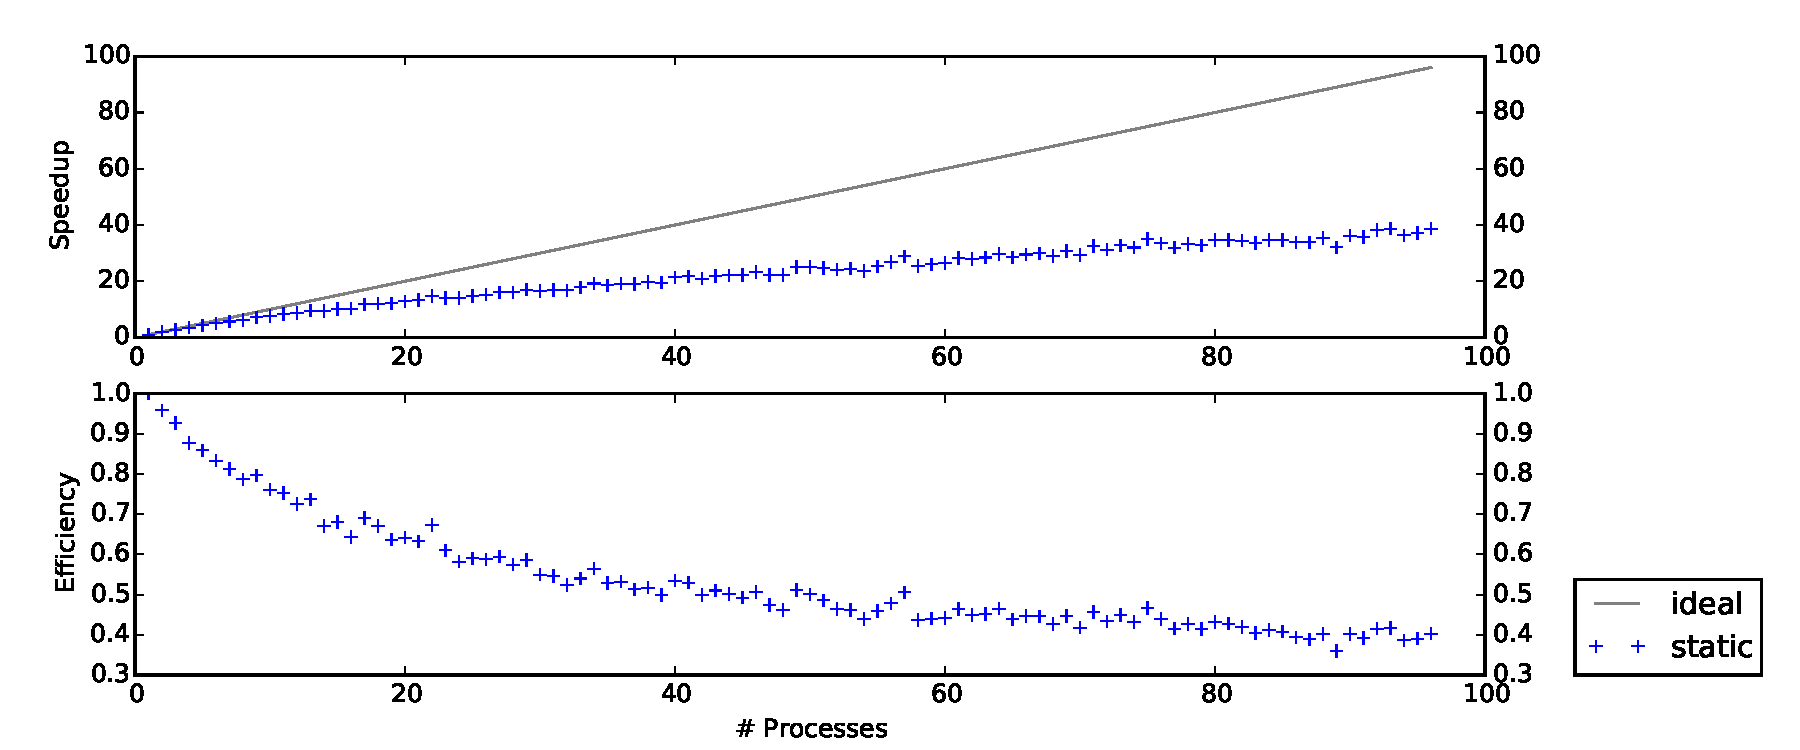
\includegraphics[width=\textwidth]
        {content/img/strong_scaling_time_static.pdf}
    \caption{Speedup bei statischer Lastverteilung}
    \label{fig:speedup_static}
\end{figure}

\begin{figure}
    \centering
    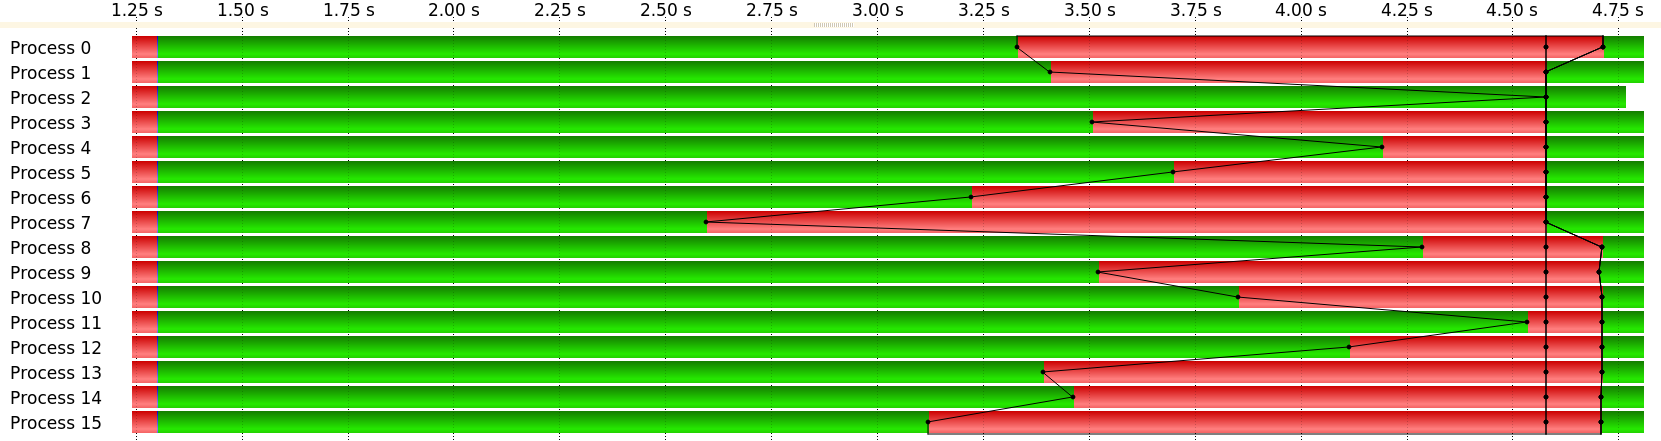
\includegraphics[width=\textwidth]
        {content/img/vampir_static.png}
        \caption{Prozess Timeline bei statischer Lastverteilung}
    \label{fig:vampir_static}
\end{figure}

In Abbildung \ref{fig:speedup_static} ist zu erkennen, dass die erreichte
Effizienz bei 96 Prozessen nur einen Wert von ungefähr \num{0,4} erreicht.
Dies liegt deutlich unter den erwarteten Werten. Eine Analyse mit Vampir \cite{vampir}
(Abbildung \ref{fig:vampir_static}) zeigt, dass eine Lastungleichheit zwischen den
Prozessen herrscht. Diese ist dadurch zu erklären, dass Spiele unterschiedlich
lange dauern. Die Länge eines Spiels wurde nach oben beschränkt: Nach 1024
Zügen wird es abgebrochen und die Punkte werden ausgezählt. Mindestens zwei
Züge sind notwendig, um ein Spiel zu beenden, da zweifaches Passen zum
Spielende führt.
Da die neuronalen Netze zufällig erstellt wurden und nach jeder Generation
zufällig verändert werden, ist es uns nicht möglich vorherzusagen, wie lange ein
Spiel zwischen zwei bestimmten Netzen dauernd wird.

\subsection{Dynamische Verteilung}

Gelöst wurde das oben beschriebene Problem der Lastungleichheit durch eine
dynamische Verteilung der Spiele auf die Prozesse.  Ein Masterprozess übernimmt
die Aufgabenverteilung, während die restlichen Workerprozesse, die Berechnungen
durchführen.  Zunächst wird ein Teil aller Spiele gleichmäßig auf alle
Workerprozesse verteilt. Ist ein Worker mit seinem Anteil fertig, schickt er
eine Anfrage an den Master. Falls noch Spiele zu berechnen sind, antwortet
dieser mit einem Auftrag zu bearbeitender Spiele, andernfalls wird mit einem
leeren Auftrag geantwortet.  Der Worker bearbeitet den Auftrag oder wartet
darauf, dass die anderen ebenfalls fertig werden.  Siehe Algorithmen
\ref{alg:master} und \ref{alg:worker}.

Dieser Ansatz wurde mit zwei Parametern untersucht. Zum
einen wurde der Anteil der initial verteilten Spiele (\emph{initial}) variiert,
zum anderen die Paketgröße (\emph{chunksize}). In der Legende der Diagramme
werden diese Konfigurationen in der Form $c-i$ dargestellt, wobei $i \in
\mathbb{N} \setminus \{0\}$ die Paketgröße und $i \in [0, 1]$ den Anteil
statisch verteilter Spiele angibt.

\begin{algorithm}
    \caption{Master}
    \label{alg:master}
    \begin{algorithmic}[1]
        \Require $initial, chunksize, n$ (number of games)
        \State $start \gets n \cdot initial$
        \While {$start < n$}
            \State $msg, worker \gets $\Call{Recv}{$anyone$}
            \State \Call{Send}{$worker, (start, \min(chunksize, n - start))$}
            \State $start \gets start + chunksize$
        \EndWhile
        \For {each process $p$}
            \State $msg, worker \gets $\Call{Recv}{$anyone$}
            \State \Call{Send}{$worker, (0, 0,$ "finished")}
        \EndFor
    \end{algorithmic}
\end{algorithm}
\begin{algorithm}
    \caption{Worker}
    \label{alg:worker}
    \begin{algorithmic}[1]
        \Require $initial, chunksize, n$ (number of games)
        \State $start, chunksize \gets \Call{partition}{n \cdot initial}$
        \While {$chunksize \neq 0$}
            \For {$g \in [start, start + chunksize)$}
                \State calculate game $\#g$
                \State count the ($wins$)
            \EndFor
            \State \Call{Send}{$master$, "request work"}
            \State $start, chunksize \gets $\Call{Recv}{$master$}
        \EndWhile
    \end{algorithmic}
\end{algorithm}

\subsubsection{Paketgröße}
Da die Anzahl an Anfragen mit sinkender Paketgröße steigt, wurde vermutet, dass
es einen Punkt gibt, ab dem die weitere Verkleinerung der Pakete für mehr
Overhead sorgt, als dass sie Zeit spart.
In Abbildung \ref{fig:speedup_chunksize} sind die Speedupkurven für Paketgrößen
von 1, 5 und 10 Spielen aufgezeichnet, während \SI{50}{\percent} der Spiele
gleichmäßig verteilt wurden. Es ist zu erkennen, dass bei der feinstmöglichen
Granularität von einem Spiel pro Paket, die erreichte Effizienz am größten ist.

\begin{figure}
    \centering
    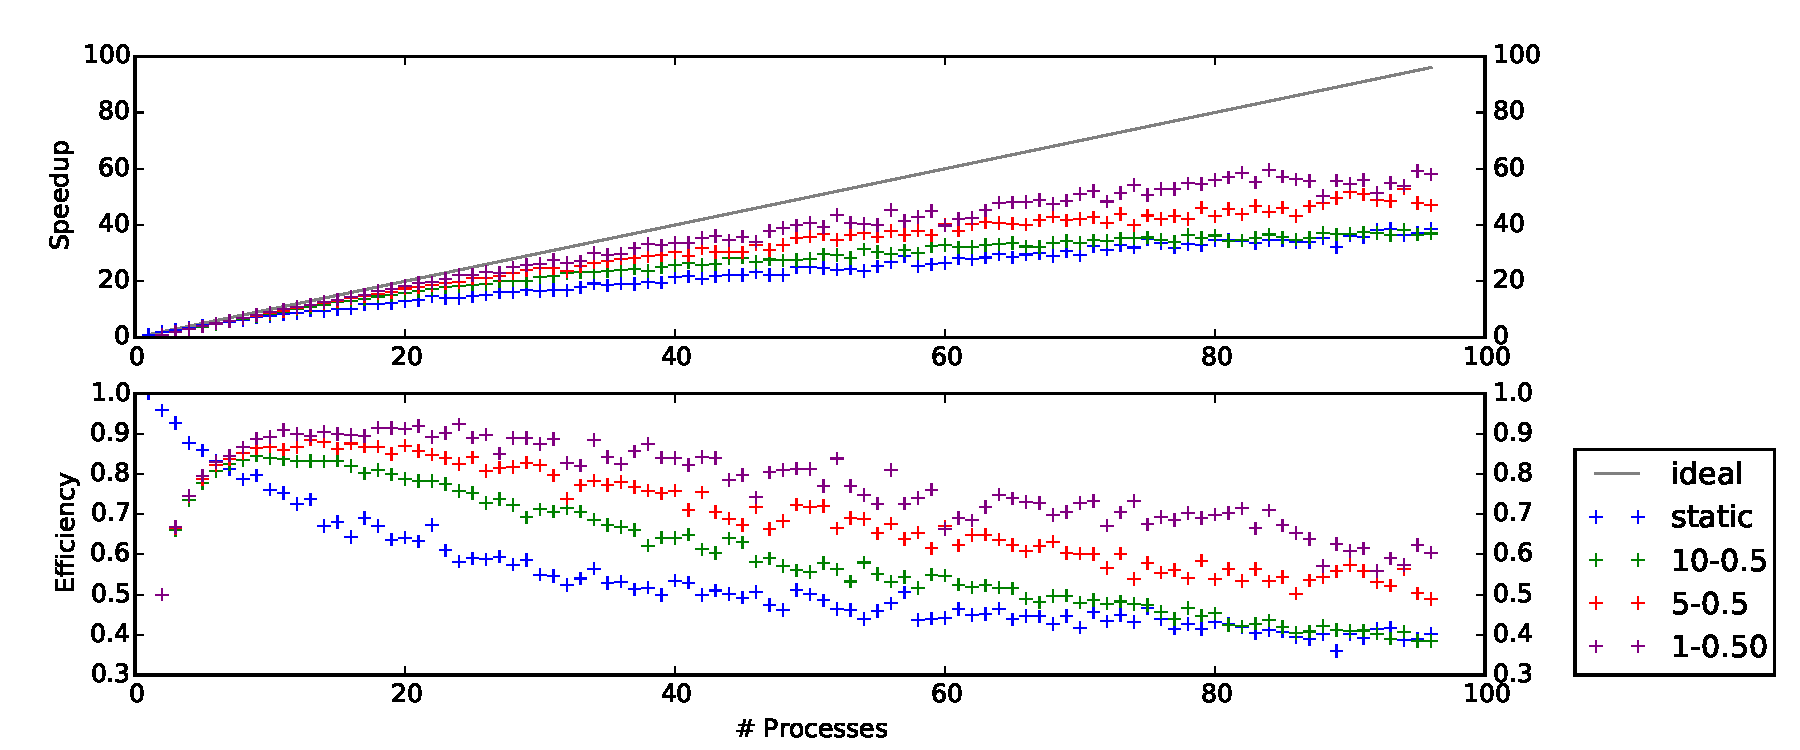
\includegraphics[width=\textwidth]
        {content/img/strong_scaling_time_chunksize.pdf}
    \caption{Vergleich von Paketgrößen}
    \label{fig:speedup_chunksize}
\end{figure}

\subsubsection{Anteil statischer Verteilung}
Der zweite Parameter gibt an, wie viele Spiele zu Beginn einer Generation
gleichmäßig auf die Worker aufgeteilt werden. Je größer der Anteil ist, desto
weniger muss über MPI kommuniziert werden. Abbildung \ref{fig:speedup_initial}
zeigt den Speedup für die initiale Verteilung von \SI{25}{\percent} bis
\SI{75}{\percent}. Je weniger statisch verteilt wurde, desto effizienter ist
die Parallelisierung. Aus Gründen der Übersichtlichkeit wurden nur drei
Konfigurationen im Diagramm aufgezeichnet. Durch Messungen wurde jedoch
festgestellt, dass initialen Verteilungen von maximal einem Drittel der Spiele
kein wesentlicher Unterschied mehr erreicht wurde.

\begin{figure}
    \centering
    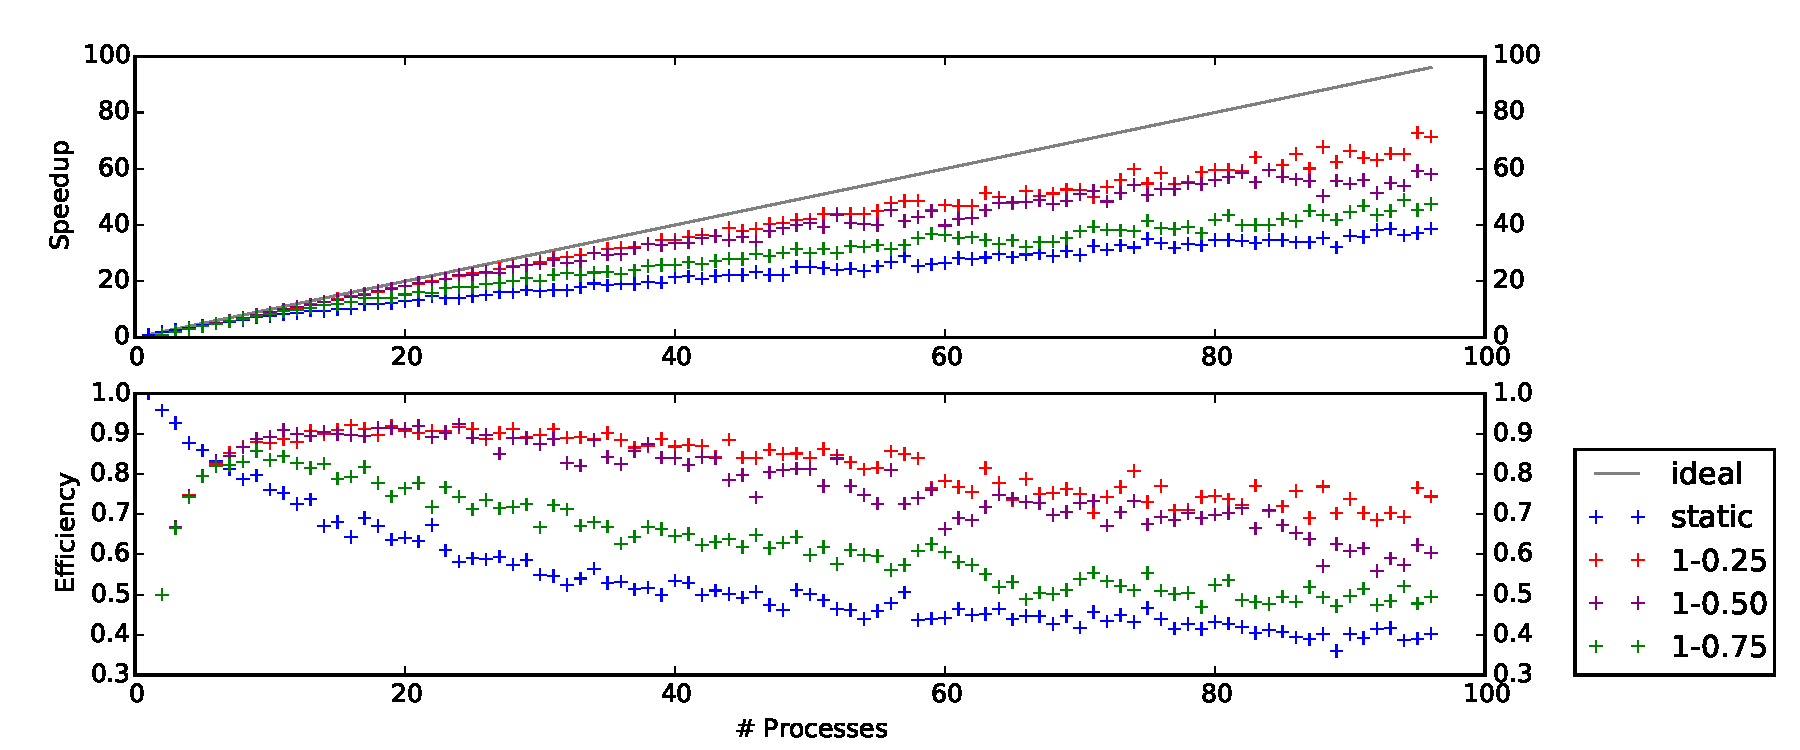
\includegraphics[width=\textwidth]
        {content/img/strong_scaling_time_initial.pdf}
    \caption{Vergleich von Anteilen der initial verteilten Spiele}
    \label{fig:speedup_initial}
\end{figure}

\subsubsection{Vergleich von dynamischer und statischer Verteilung}
Während der erste Ansatz beinahe ohne MPI-Kommunikation auskommt -- es werden
ausschließlich die Ergebnisse am Generationsende aufsummiert -- benötigt die
dynamische Verteilung pro verteiltem Paket zwei Punkt-zu-Punkt Übertragungen.
Zudem beteiligt sich der Masterprozess nicht an der Berechnung.  Dennoch kommt
es zu einem deutlichen Unterschied bezüglich Speedup und Effizienz (Abbildung
\ref{fig:speedup_final}): Mit ca. \SI{75}{\percent} Effizienz bei 96 Prozessen
erreicht die dynamische Verteilung ein wesentlich besseres Ergebnis als die
statische Aufteilung mit ca. \SI{40}{\percent}.

\begin{figure}
    \centering
    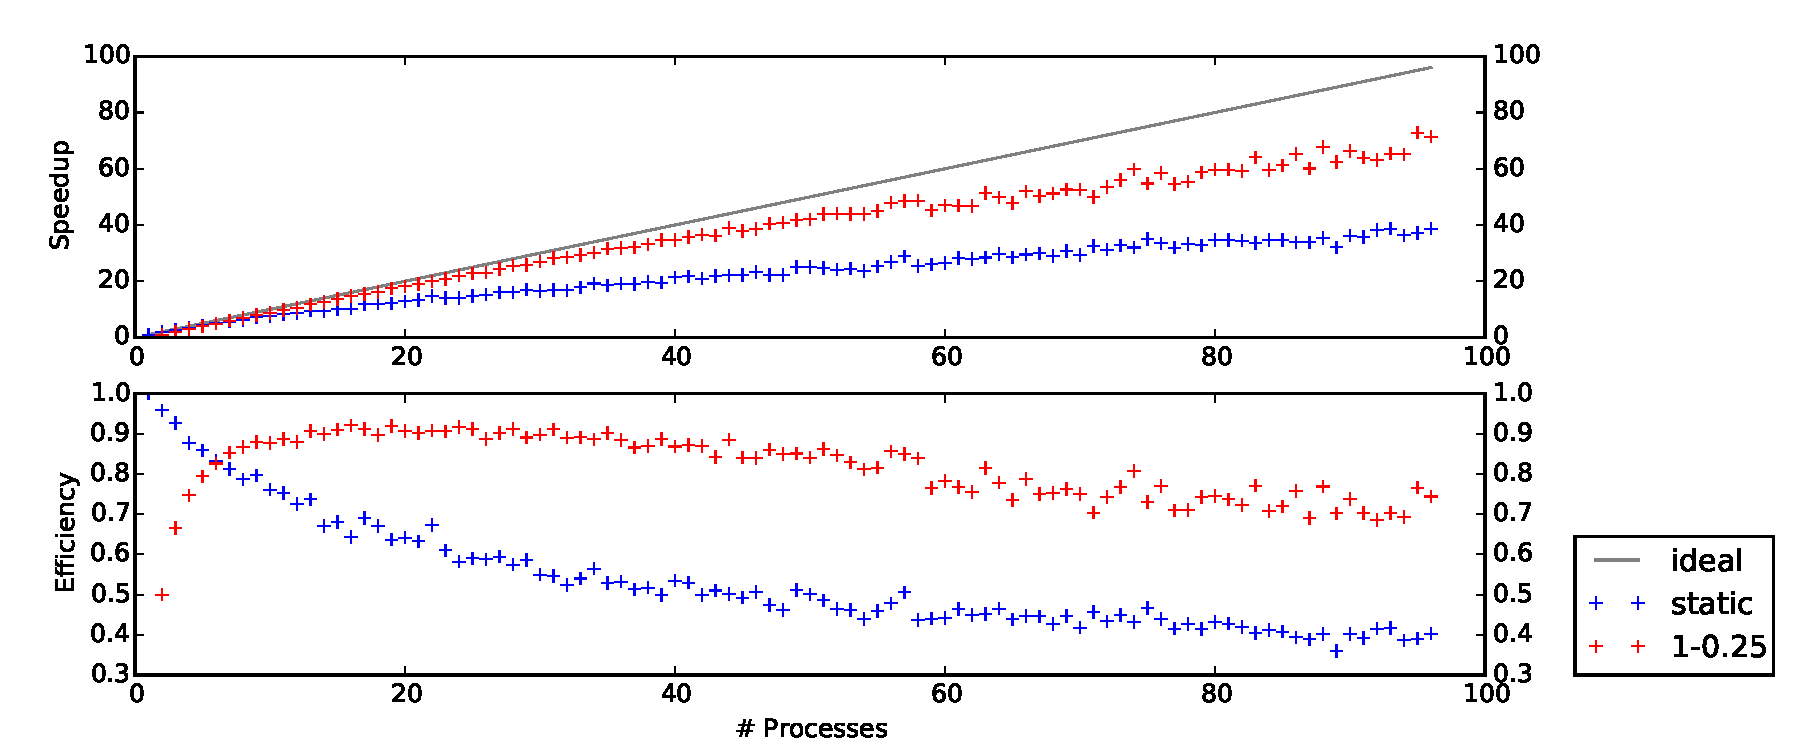
\includegraphics[width=\textwidth]
        {content/img/strong_scaling_time_final.pdf}
    \caption{Vergleich von dynamischer und statischer Lastverteilung}
    \label{fig:speedup_final}
\end{figure}

In Abbildung \ref{fig:vampir_dynamic} ist das Kommunikationsschema einer
Generation dargestellt. Der Masterprozess (Prozess 0) beantwortet ab
\SI{1,8}{\second} die eintreffenden Requests der Workerprozesse. Jeder
erkennbare Strich zwischen dem Master und einem Worker repräsentiert eine
Request und die dazugehörige Response.

\begin{figure}
    \centering
    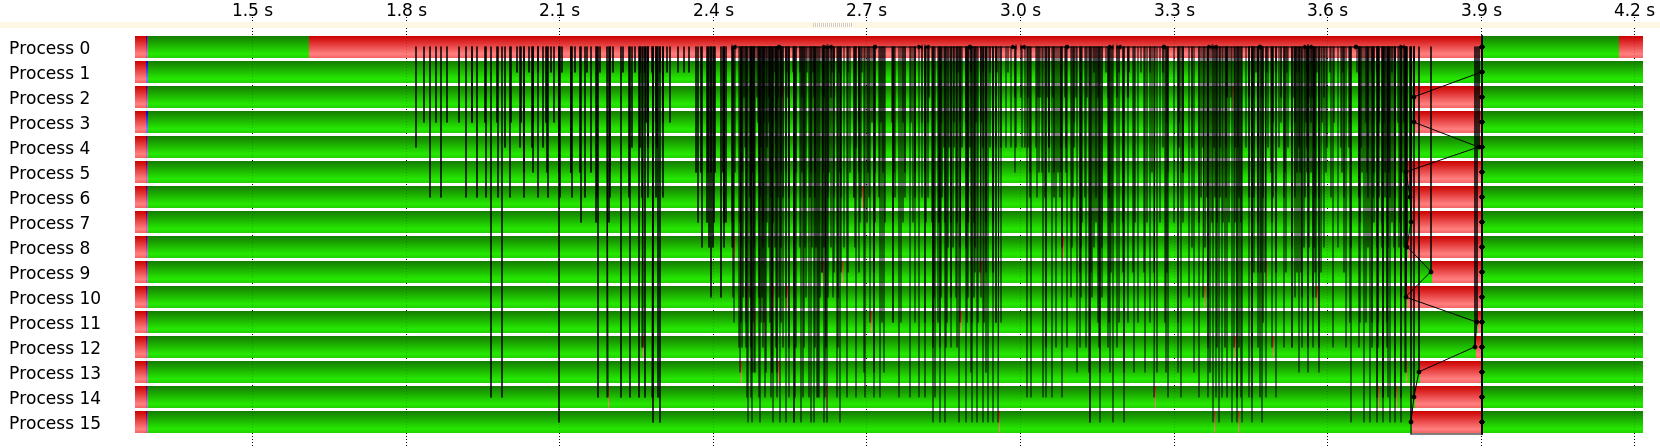
\includegraphics[width=\textwidth]
        {content/img/vampir_dynamic.png}
        \caption{Prozess Timeline bei dynamischer Lastverteilung}
    \label{fig:vampir_dynamic}
\end{figure}

Gut erkennbar sind die unterschiedlichen Längen der Spiele. Die grün
dargestellten Bereiche zwischen den MPI-Aufrufen auf den Balken der Worker
zeigen jeweils die Berechnung eines Spiels. Betrachtet man beispielsweise den
Prozess 15. Das erste vom Master zugeteilte Spiel wird ab \SI{2,1}{\second}
berechnet und braucht ungefähr \SI{0,2}{\second}. Anschließend bei ca.
\SI{2,3}{\second}, kommuniziert Prozess 15 zweimal kurz hintereinander mit dem
Master. In dem Intervall zwischen den beiden Anfragen wird ein weiteres Spiel
berechnet.

Die Antwortzeit bei den Anfragen ist im Vergleich zu der Zeit, welche für die
Berechnung eines Spiels aufgewendet wird, so gering, dass die Wartezeit für die
Worker vernachlässigbar gering bleibt. Auch die Wahrscheinlichkeit für
gleichzeitige Anfragen von mehreren Prozessen ist gering genug, so dass mit
synchronen Sende- und Empfangsinstruktionen gearbeitet werden kann.

Die Lastungleichheit ist weitestgehend behoben. Zum Ende der Generation muss
zwar noch gewartet werden, jedoch ist die Ausnutzung der verfügbaren Rechenzeit
im Vergleich zu der vorherigen Situation deutlich besser.

\subsection{Hybride Parallelisierung}
Zusätzlich zu obigem Parallelisierungsschema wurde hybride Parallelisierung mit
MPI und OpenMP ausprobiert.  Dabei wurde untersucht, wie sich die Aufteilung
der Schleifen in der Ausgabeberechnung der neuronalen Netz auf
verschiedene Threads verhält.

In der Testkonfiguration wurde ein rechnender MPI-Prozess mit OpenMP-Threads
gestartet, so dass jeder Thread auf einem eigenen Prozessorkern läuft.  Mit
einem einzelnen Thread -- also sequentiell -- lag die Laufzeit deutlich über
der, der entsprechenden Variant ohne OpenMP.  Mit jedem zusätzlichen Thread
stieg die Laufzeit weiter an. Daher wurde dieser Ansatz wieder verworfen und
sich auf einen MPI-Prozess pro Prozessorkern beschränkt.

Zwar wird viel Rechenzeit in \texttt{nnnet\_calculate\_output} verbracht, aber
wir vermuten, dass Berechnung einer einzelnen Ausgabe schnell genug ist, so
dass der Overhead beim Erstellen und Zerstören der Threads gegenüber der
eingesparten Rechenzeit deutlich überwiegt. Da bei jedem Zug eine Ausgabe
berechnet wird resultieren viele und lange Spiele einer anteilig hohen
Benutzung dieses Codeabschnitts.

\section{Die Ergebnisse}
%Funktioniert es? Wie ist der Zeitaufwand? Was heißt das für Go mit neuroonalen
%Netzen?hg
Das bisherige Ergebnis war etwas ernüchternd. Die trainierten Netze spielen in
der Regel besser, als untrainierte, aber auch das beste Netz (gemessen nach
Siegen gegen andere, gleich viel trainierte) hat keine Chance gegen einen 
Menschen, sofern dieser halbwegs überlegt spielt.
Für die Tragweite von Neuronalen Netzen, im Hinblick auf die Kompetenz Go gut
spielen zu können, hat dies allerdings wenig zu Bedeuten. In diesem Projekt
haben wir lediglich eine von vielen Arten von Neuronalen Netzen benutzt, wobei
nicht klar ist, ob diese Art die best geeignetste ist. Zusätzlich dazu gibt es
in diesem Ansatz viele Parameter, die durch teilweise Abänderung mit Sicherheit 
einen positiven Effekt auf die Performance der Netze hätten. 
\section{Fazit}

Die Spielleistung der trainierten neuronalen Netze war nicht überragend. Für
ein besseres Ergebnis in dieser Hinsicht, hätte man sich mehr mit der Theorie
hinter neuronalen Netzen beschäftigen müssen. Auch weitere Erfahrung in Bezug
auf Computer Go wäre sicherlich nützlich gewesen.

Da der Titel des Praktikum „Parallele Programmierung“ lautet, war die
Beschäftigung mit dem Thema der künstlichen Intelligenz nur ein Nebenprodukt.
Die im Vordergrund stehende Parallelisierung des Programms war insofern ein
Erfolg, dass wir ein naives, nur mäßig effizientes, Parallelisierungsschema
analysiert und die Schwachstellen erkannt haben.  Mittels den gewonnenen
Erkenntnissen wurde erfolgreich ein alternatives Schema entworfen und
implementiert. Dieses lieferte einen, in unseren Augen, akzeptablen
Speedup. Interessant an der Parallelisierung war, dass sich die zu verteilende
Last nicht vorhersehbar änderte und daher dynamisch, während der Laufzeit
darauf eingegangen werden musste.


\clearpage

\begin{appendices}

\section{Verwendete Software}

Für unsere Anwendung haben wir die folgende Software verwendet:

Compiler
\begin{itemize}
    \item GNU Compiler Collection \cite{gcc}
\end{itemize}

Libraries
\begin{itemize}
    \item GNU C Library \cite{glibc}
    \item OpenMPI \cite{openmpi}
    \item GNU Readline \cite{readline}
    \item Check \cite{check}
\end{itemize}

Tools
\begin{itemize}
    \item Git \cite{git}
    \item CMake \cite{cmake}
    \item Doxygen \cite{doxygen}
    \item Vampir \cite{vampir}
\end{itemize}

Dieser Bericht wurde mit {\LaTeX} und {\KOMAScript} erstellt. Die Diagramme
wurden mit matplotlib \cite{matplotlib} erstellt.

\end{appendices}


\clearpage

\printbibliography[heading=bibintoc]

\listoffigures
\lstlistoflistings


\end{document}
